\documentclass{beamer}
\usetheme{Warsaw}
\usecolortheme{penn}

% Penn official colors: Blue #011F5B, Red #990000
% beamercolorthemepenn.sty loaded from CTAN (beamertheme-upenn-bc package)

\usepackage{booktabs}
\usepackage{graphicx}
\usepackage{amsmath}
\usepackage{xcolor}

% Penn blue for blocks and alerts
\definecolor{pennblue}{HTML}{011F5B}
\definecolor{pennred}{HTML}{990000}

\setbeamercolor{alerted text}{fg=pennred}
\setbeamercolor{block title}{bg=pennblue, fg=white}
\setbeamercolor{block body}{bg=pennblue!8, fg=black}

\title[Cross-Dataset HAR Transfer]{Physics-Grounded Data Augmentation\\Outperforms Model Adaptation\\for Cross-Dataset HAR Transfer}

\author{Gengzhan \and Forest \and Gengzhan}
\institute{University of Pennsylvania}
\date{April 2026}

\begin{document}

% ---- Slide 1: Title ----
\begin{frame}
\titlepage
\end{frame}

% ---- Slide 2: Motivation ----
\begin{frame}{Motivation: Models Don't Travel Well}

\begin{block}{The Problem}
Train a HAR classifier on UCI HAR $\rightarrow$ deploy on WISDM \\
\medskip
\textbf{Result: F1 = 0.085} (near random chance for 5 classes)
\end{block}

\bigskip
Why? The two datasets use:
\begin{itemize}
    \item Different sensor placements (waist vs.\ front pocket)
    \item Different sampling rates (50\,Hz vs.\ 20\,Hz)
    \item Different signal processing (filtered vs.\ raw)
\end{itemize}

\bigskip
\textbf{Domain shift is the culprit.}\\
The question is: \emph{which kind of domain shift, and can we fix it?}

\end{frame}

% ---- Slide 3: Two Datasets ----
\begin{frame}{Two Very Different Datasets}

\begin{table}
\centering
\begin{tabular}{lcc}
\toprule
Property & UCI HAR & WISDM v1.1 \\
\midrule
Placement & Waist (fixed) & Front pocket (free) \\
Sampling rate & 50\,Hz & 20\,Hz \\
Filtering & Butterworth LP & None (raw) \\
Subjects & 30 & 36 \\
Training windows & 8,355 & --- \\
Test windows & --- & 5,307 \\
Units & m/s$^2$ & m/s$^2$ \\
Window size (aligned) & \multicolumn{2}{c}{$51 \times 3$ @ 20\,Hz} \\
\bottomrule
\end{tabular}
\end{table}

\bigskip
Same activity classes, but the sensor sees the world very differently.

\end{frame}

% ---- Slide 4: 7 Sources of Domain Shift ----
\begin{frame}{Seven Sources of Domain Shift}

\begin{table}
\centering
\small
\begin{tabular}{clc}
\toprule
Rank & Source & Magnitude \\
\midrule
\textcolor{red}{\textbf{1}} & \textcolor{red}{\textbf{Gravity axis projection}} & \textcolor{red}{\textbf{$W_1 = 8.7$\,m/s$^2$}} \\
2 & Signal dynamic amplitude & 3--5$\times$ difference \\
3 & Noise temporal structure & AR(1) $\alpha \approx 0.986$ vs.\ white \\
4 & Class prior distribution & TVD $= 0.36$ \\
5 & Gait spectral energy (0.8--2\,Hz) & WISDM $+40\%$ \\
6 & Inter-subject variability & $W_1^{\max} = 1.89$\,m/s$^2$ \\
7 & Gravity magnitude attenuation & 9.69 vs.\ 7.29\,m/s$^2$ \\
\bottomrule
\end{tabular}
\end{table}

\bigskip
\textcolor{red}{\textbf{Gravity axis mismatch completely dominates.}}

\end{frame}

% ---- Slide 5: Dominant Shift - Gravity Axis ----
\begin{frame}[shrink=8]{Dominant Shift: Gravity Axis Projection}

\begin{columns}[T]
\begin{column}{0.52\textwidth}
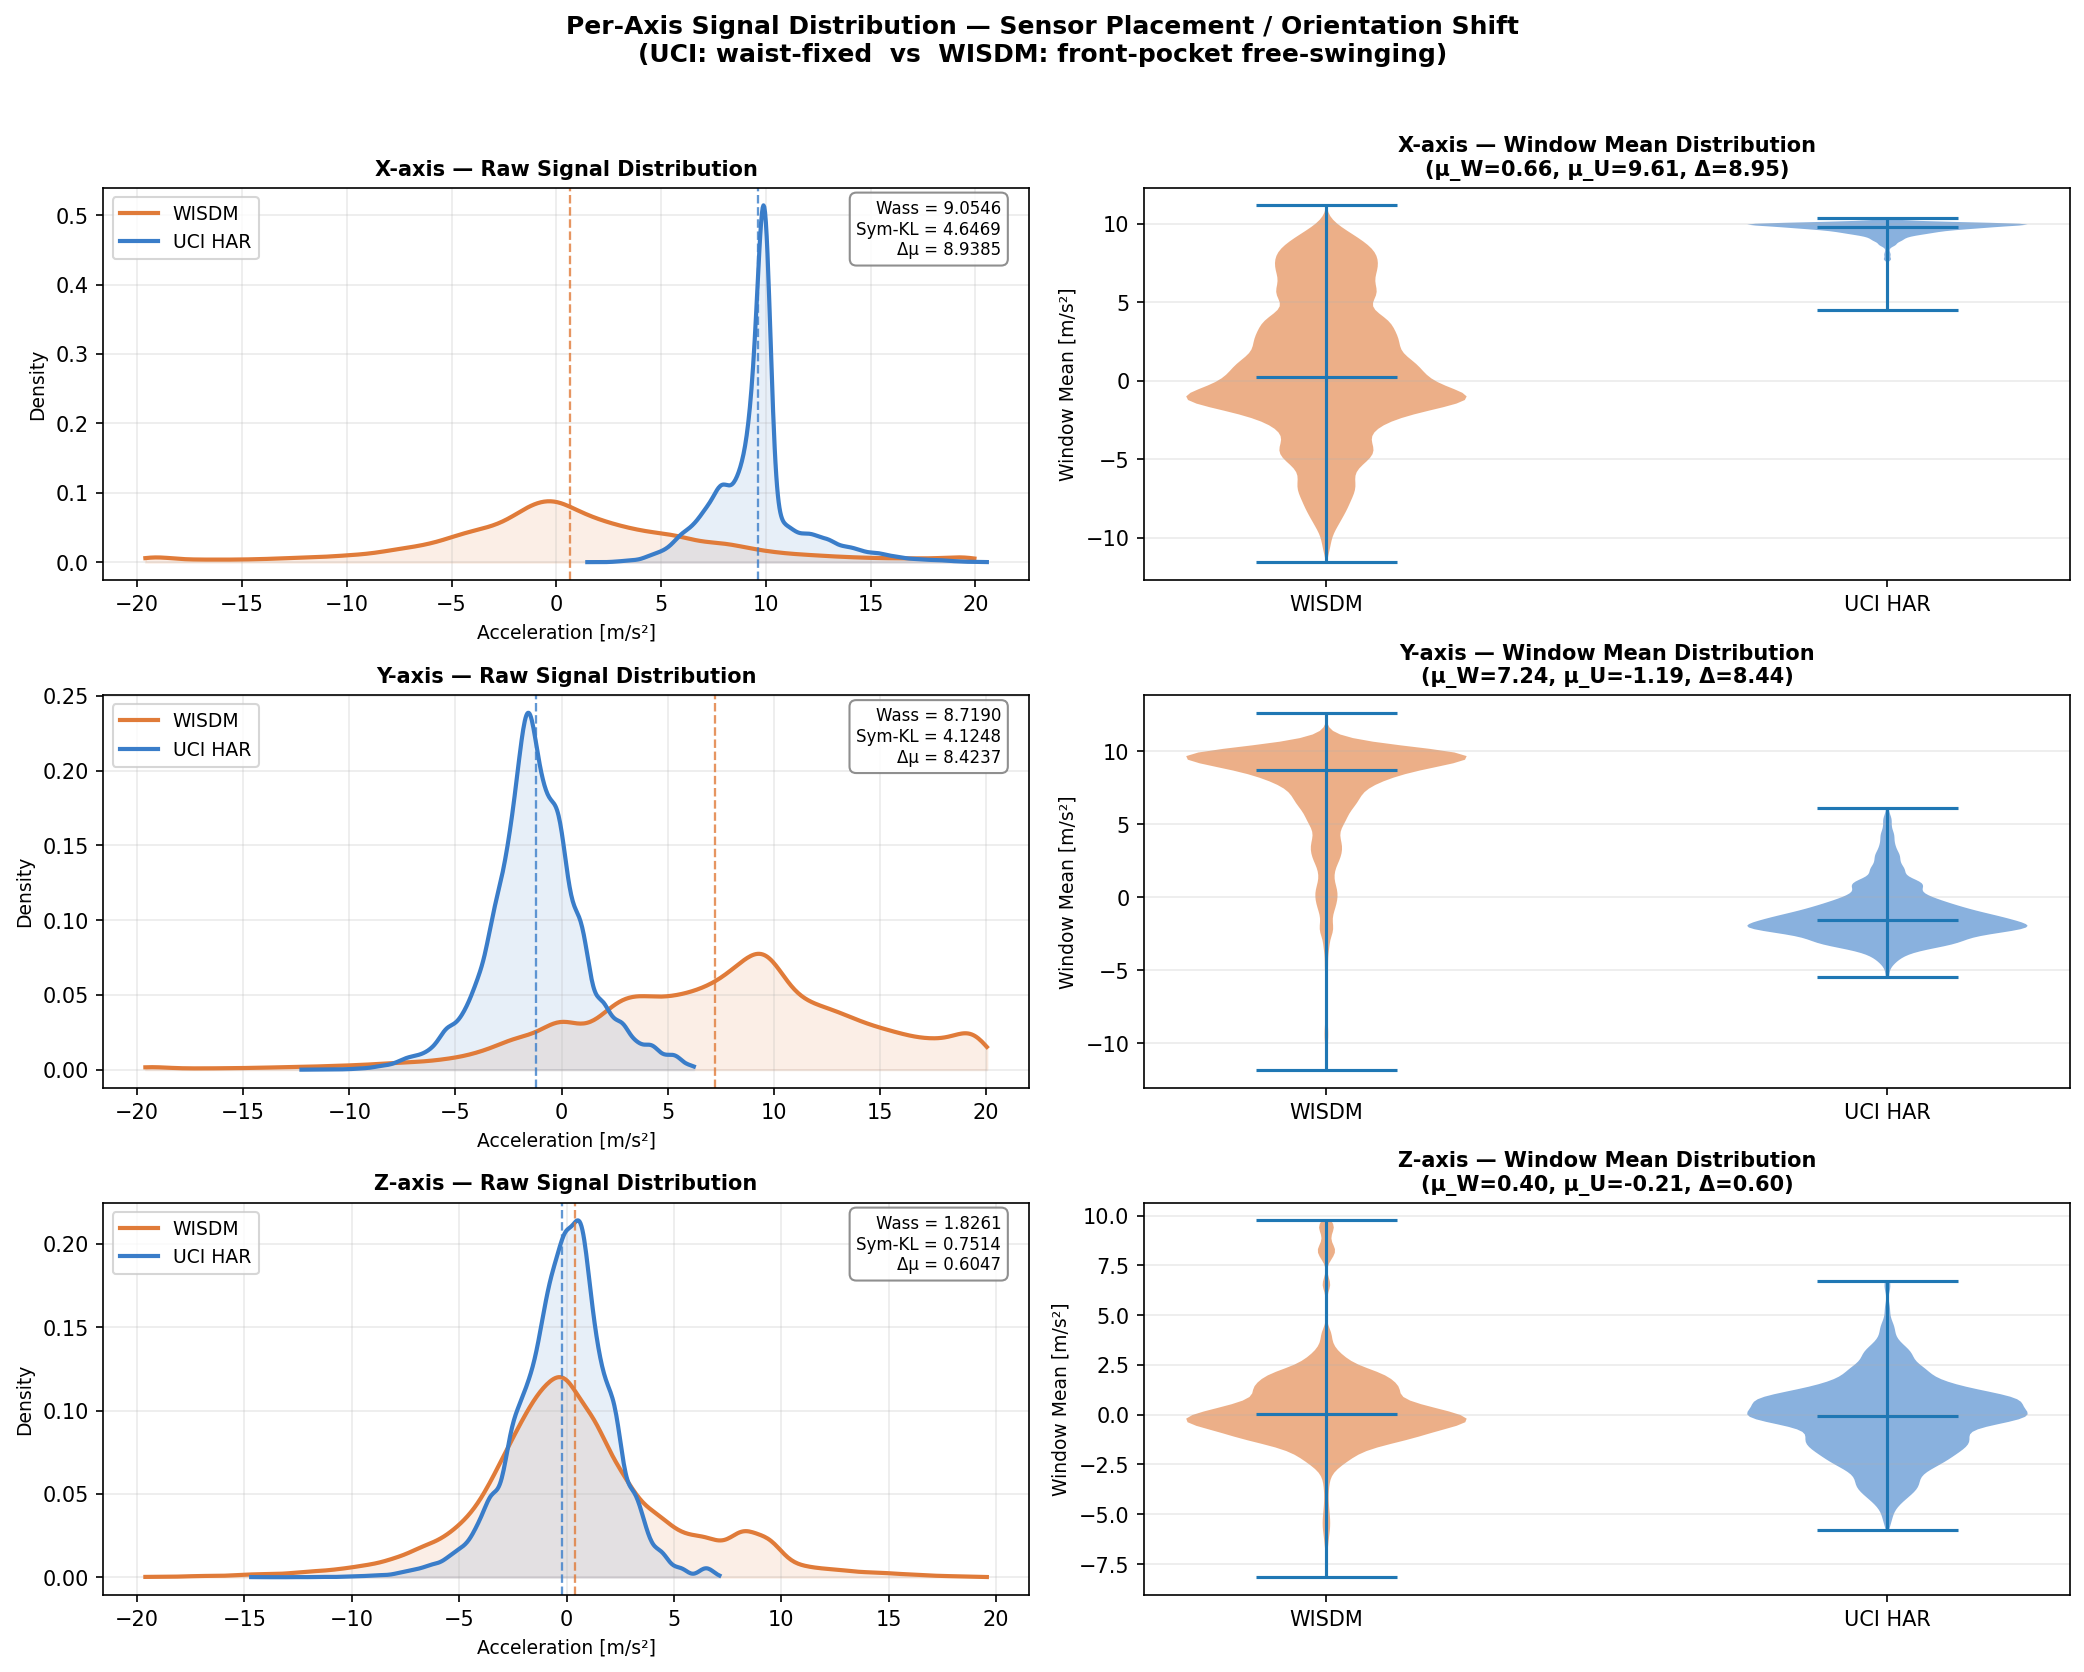
\includegraphics[width=\textwidth]{figures/per_axis_analysis.png}
\end{column}
\begin{column}{0.44\textwidth}
\textbf{What's happening:}
\begin{itemize}
    \item Waist mount: gravity $\to$ \textbf{X-axis}\\
    Mean $= +8.58$\,m/s$^2$
    \item Front pocket: gravity $\to$ \textbf{Y-axis}\\
    Mean $= +6.51$\,m/s$^2$
    \item X-axis $W_1 = \mathbf{8.7}$\,m/s$^2$
\end{itemize}

\smallskip
Sensor is physically rotated ${\sim}90^\circ$.

\smallskip
A model trained on UCI HAR learns ``X has big DC.'' In WISDM, X is near zero-mean. This is why raw transfer fails.
\end{column}
\end{columns}

\end{frame}

% ---- Slide 6: Shift in Feature Space ----
\begin{frame}{How Bad Is the Gap in Feature Space?}

\begin{center}
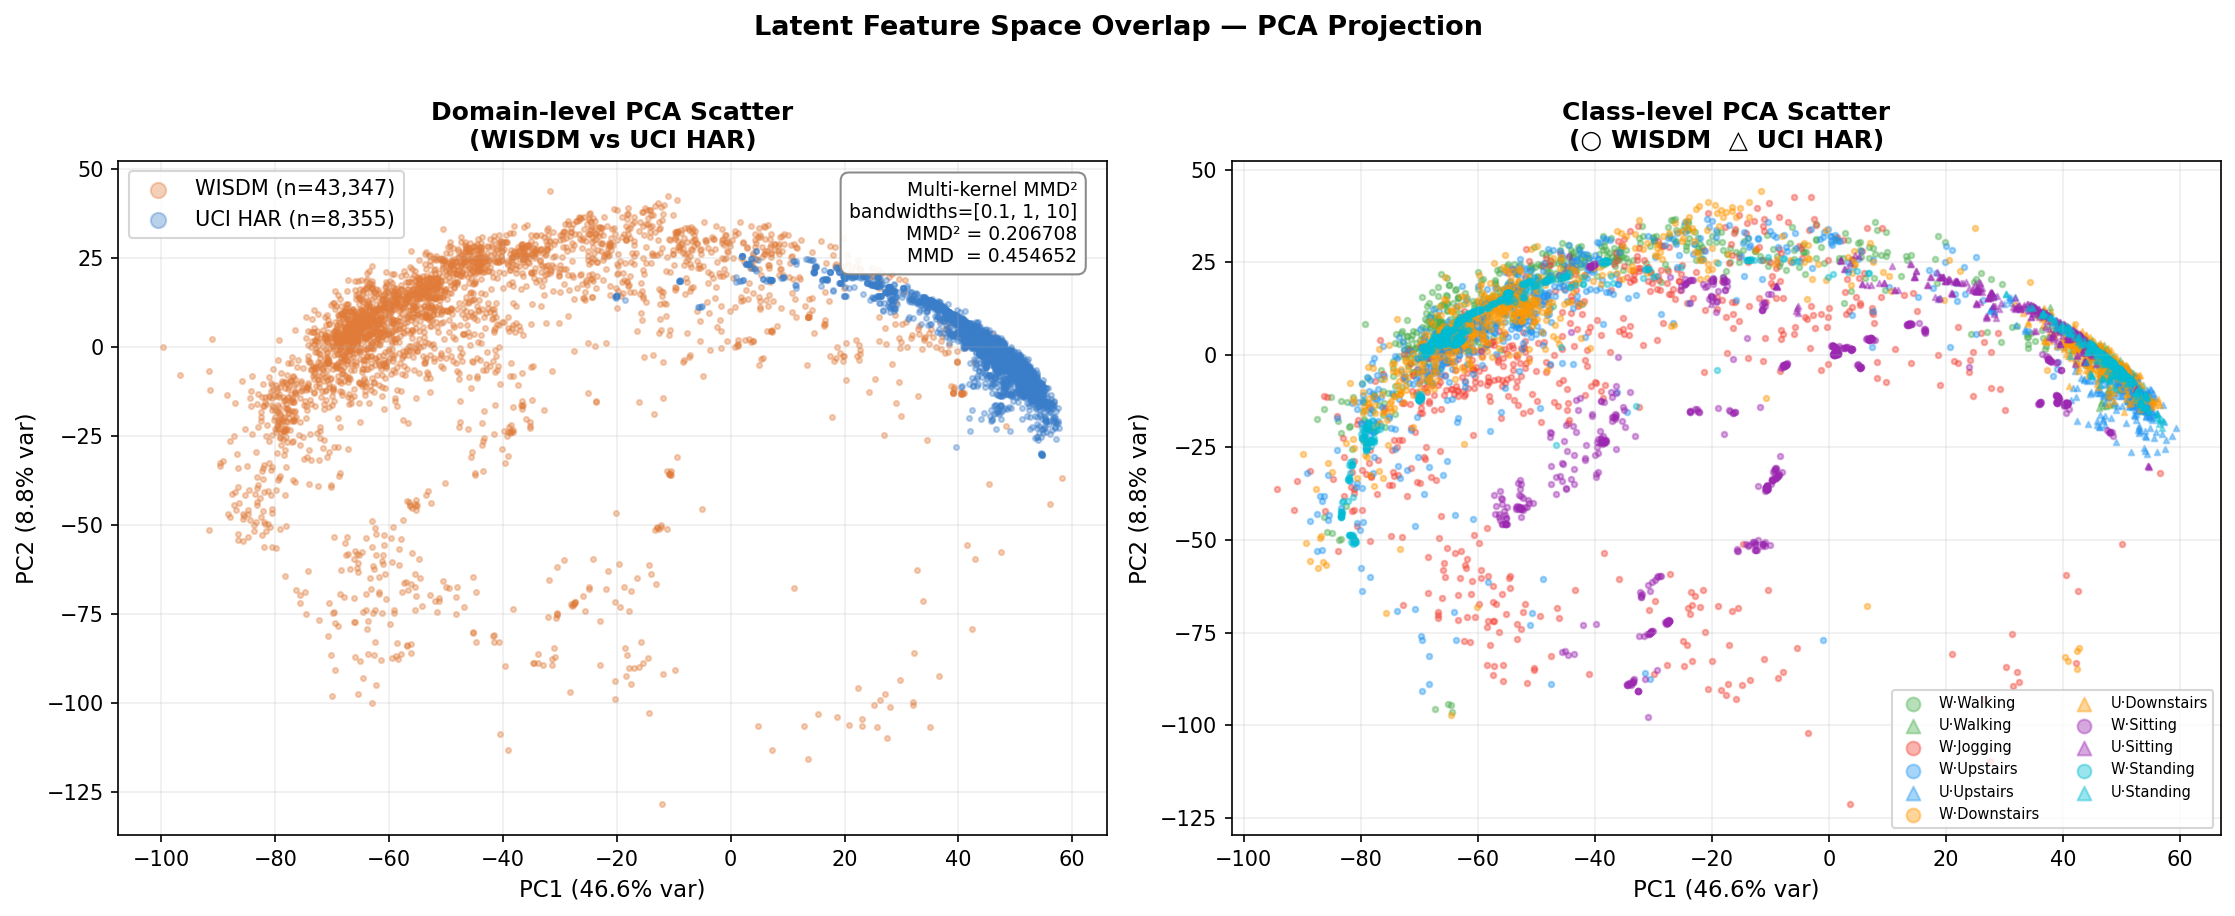
\includegraphics[width=0.92\textwidth]{figures/latent_space_overlap.png}
\end{center}

\smallskip
\textbf{Multi-kernel MMD = 0.830} \quad Two datasets barely overlap. Raw transfer has no chance.

\end{frame}

% ---- Slide 7: Adaptation Strategy - PhysicalDistortion ----
\begin{frame}{Our Approach: PhysicalDistortion}

Instead of adapting the model, we transform the \emph{data}.

\medskip
\textbf{Five-operator pipeline applied to UCI HAR training data:}

\begin{enumerate}
    \item \textbf{Orientation shift}: rotate 90$^\circ$ around Z + random wobble $\pm 10^\circ$
    \item \textbf{Gravity attenuation}: scale by $0.7523 = 7.29 / 9.69$
    \item \textbf{Per-activity amplitude scaling}: empirical per-axis scale factors (not global)
    \item \textbf{Gait spectral boost}: $\times$Uniform[1.2, 1.5] in 0.8--2\,Hz band (locomotion only)
    \item \textbf{AR(1) colored noise}: $\alpha = 0.9865$, initialized from stationary distribution
\end{enumerate}

\medskip
Each operator targets a specific, \emph{measured} physical difference.\\
No target labels used. No model architecture changes.

\end{frame}

% ---- Slide 8: Results After Alignment ----
\begin{frame}{After PhysicalDistortion: Distributions Align}

\begin{center}
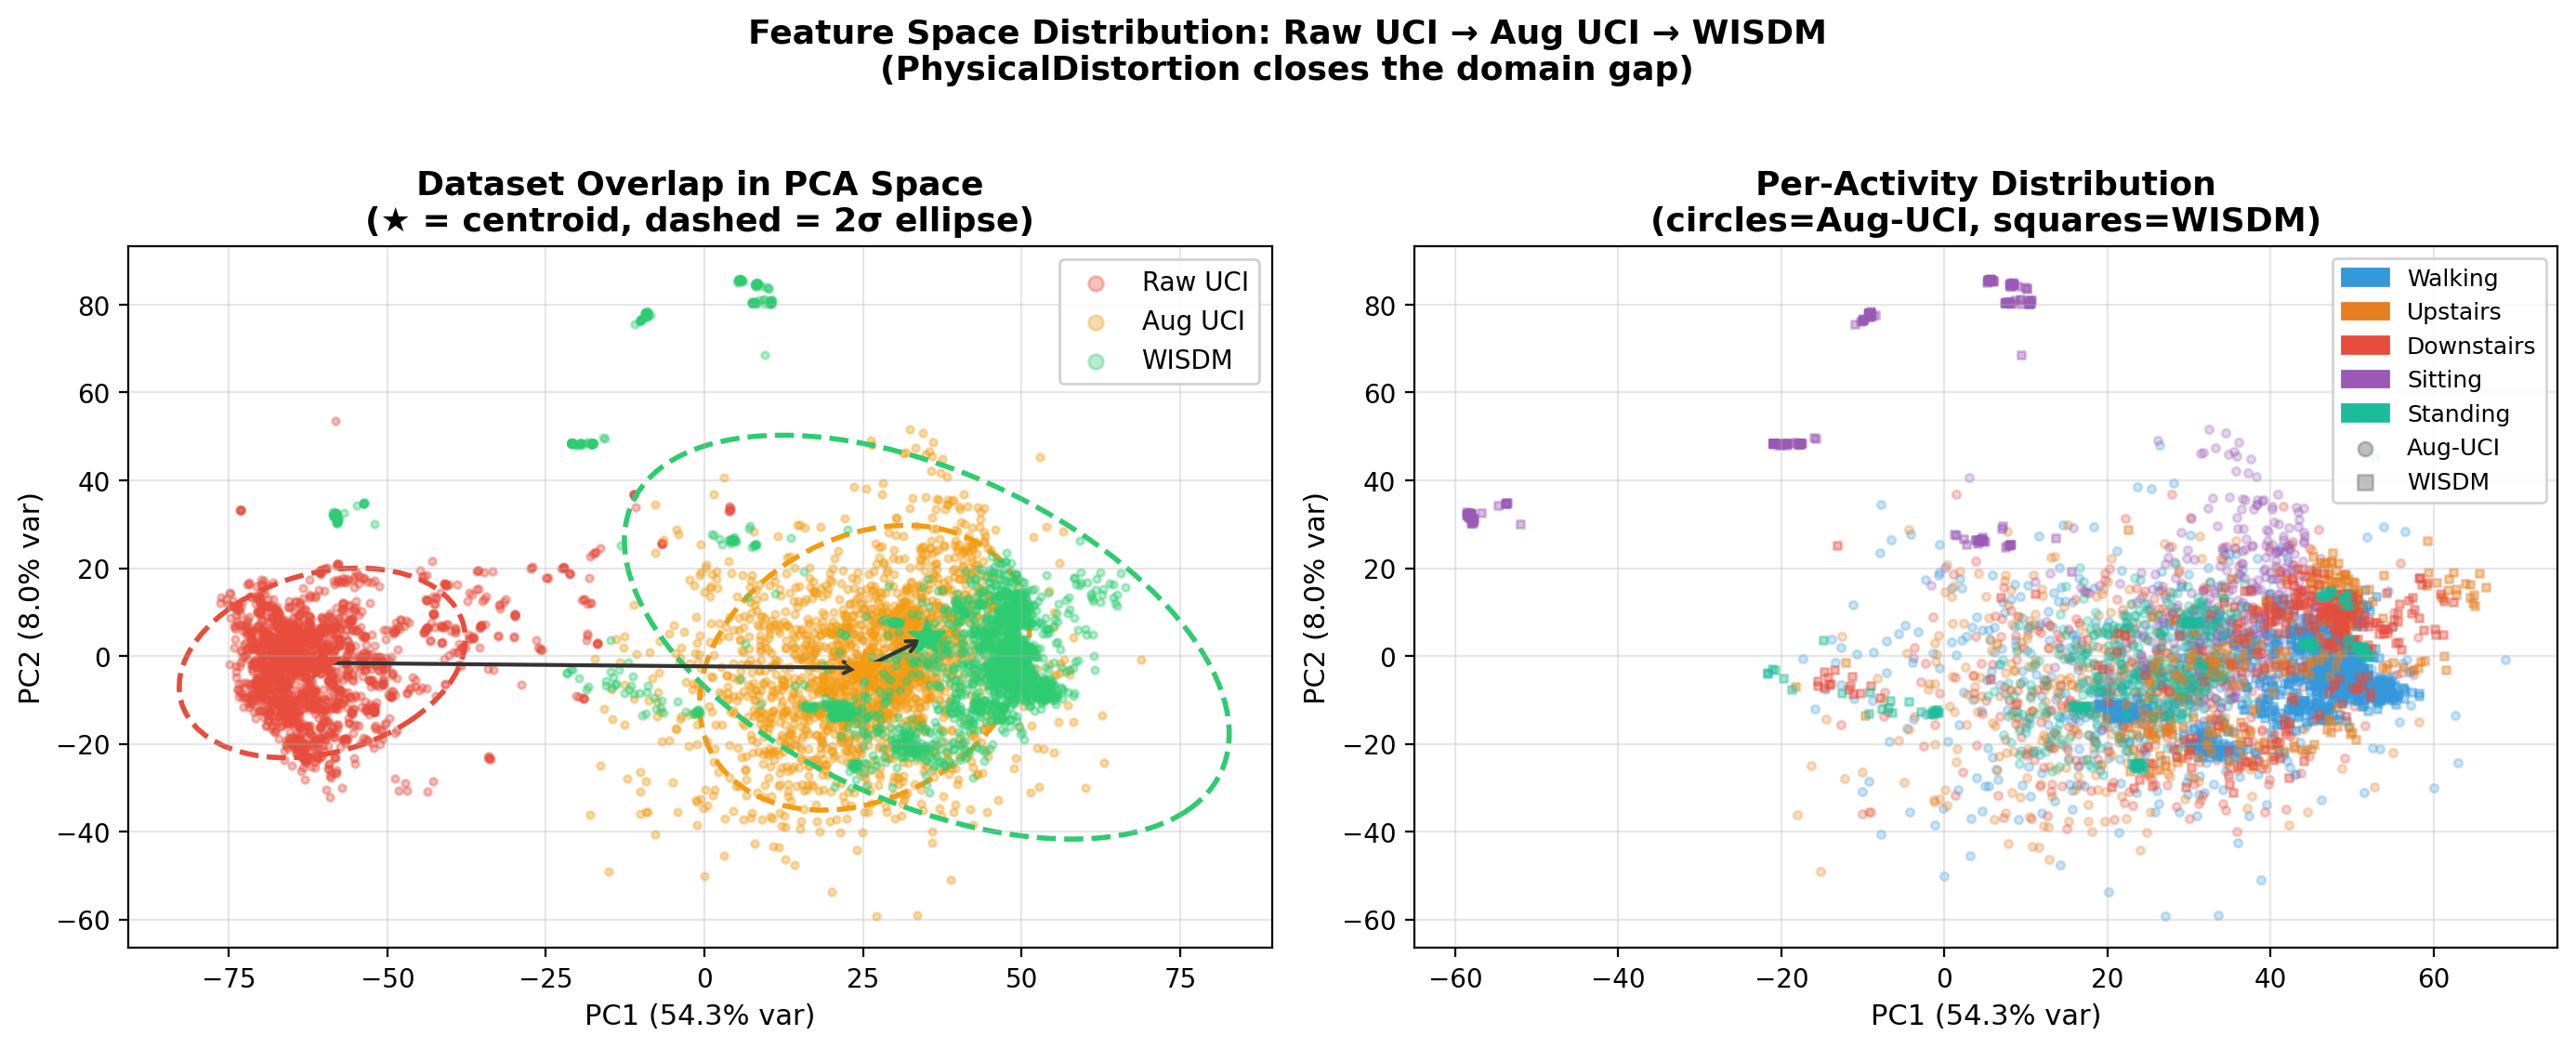
\includegraphics[width=0.92\textwidth]{figures/distribution_alignment.png}
\end{center}

\smallskip
\textbf{MMD: $0.830 \rightarrow 0.453$} \quad (45.4\% reduction) \quad Gap shrinks but doesn't close — explains remaining per-class failures.

\end{frame}

% ---- Slide 9: Ablation Results ----
\begin{frame}{Ablation: Four Conditions, Five Architectures}

\begin{table}
\centering
\small
\begin{tabular}{lcccc}
\toprule
Model & C0 Raw & C1 Distort & C2 +TTBN & C3 +DANN \\
\midrule
CNN1D       & 0.120 & \textbf{0.723} & 0.610 & 0.581 \\
Transformer & 0.046 & \textbf{0.580} & 0.580 & 0.327 \\
FFN         & 0.069 & \textbf{0.542} & 0.425 & 0.401 \\
TCN         & 0.127 & \textbf{0.535} & 0.451 & 0.418 \\
BiGRU       & 0.062 & \textbf{0.512} & 0.512 & 0.365 \\
\midrule
Average     & 0.085 & \textbf{0.578} & 0.516 & 0.418 \\
\bottomrule
\end{tabular}
\end{table}

\bigskip
\begin{itemize}
    \item C0 Raw: essentially random ($6.8\times$ improvement from C1)
    \item \textbf{C1 is best across every architecture}
    \item TTBN and DANN both \textcolor{red}{hurt} compared to C1 alone
\end{itemize}

\end{frame}

% ---- Slide 10: Per-class Analysis ----
\begin{frame}{Per-class Analysis: Honest Look}

\begin{columns}[T]
\begin{column}{0.52\textwidth}
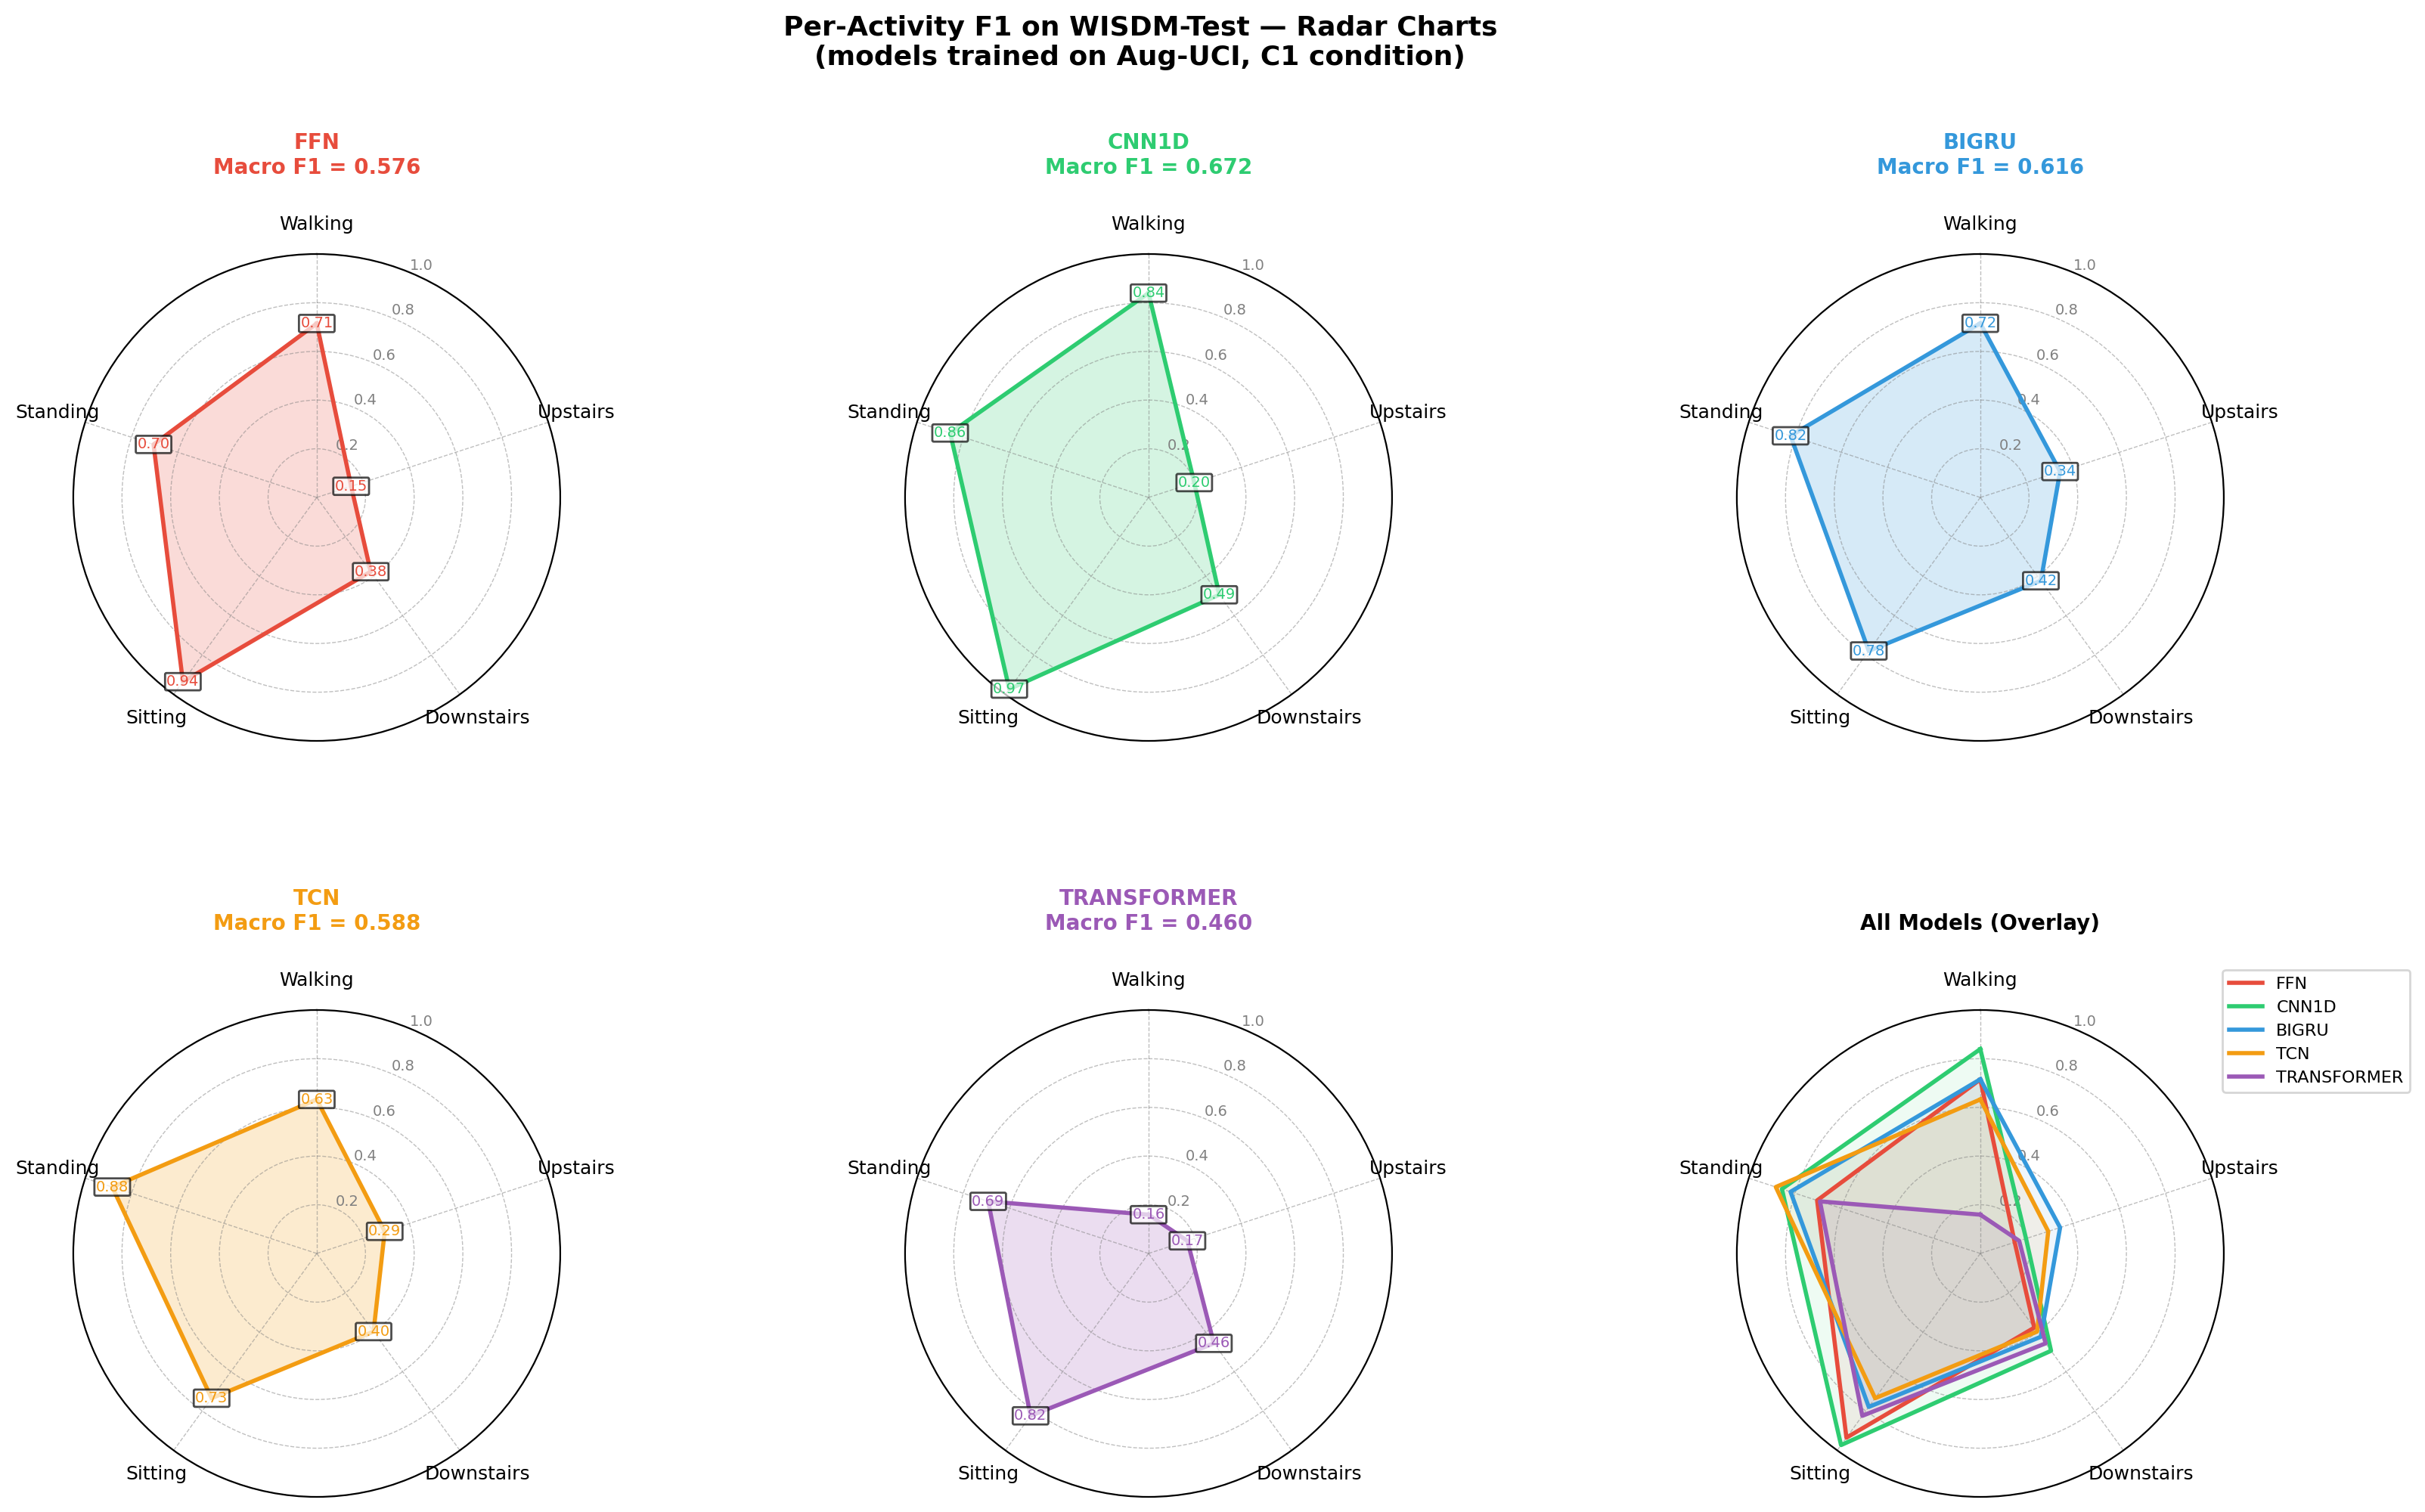
\includegraphics[width=0.95\textwidth]{figures/radar_charts.png}
\end{column}
\begin{column}{0.44\textwidth}
\textbf{CNN1D, C1 condition:}

\medskip
\begin{tabular}{lc}
\toprule
Activity & F1 \\
\midrule
Walking    & 0.872 \\
Sitting    & 0.966 \\
Standing   & 0.820 \\
Downstairs & 0.513 \\
\textcolor{red}{Upstairs}   & \textcolor{red}{0.445} \\
\bottomrule
\end{tabular}

\bigskip
Static activities: nearly perfect.\\[4pt]
\textcolor{red}{Upstairs is a real failure.}\\
Step patterns vary a lot across subjects and sensor wobble is hard to correct at window level.
\end{column}
\end{columns}

\end{frame}

% ---- Slide 11: Why TTBN/DANN Don't Help ----
\begin{frame}[shrink=12]{Why TTBN and DANN Don't Help}

\textbf{After PhysicalDistortion, model-level adaptation makes things worse.}

\medskip
\textbf{TTBN fails because:}
\begin{itemize}
    \item Re-estimates BN stats from test batches
    \item WISDM is class-imbalanced (Walking = 56\% vs.\ UCI 20\%, TVD = 0.36)
    \item Small test batches give noisy estimates that push stats in wrong direction
\end{itemize}

\smallskip
\textbf{DANN fails because:}
\begin{itemize}
    \item Forces domain-invariant features
    \item But the shift is tied to activity itself (gravity projection differs per activity)
    \item Invariance destroys axis-specific information the classifier needs
    \item Training is also unstable; adversarial loss weight is hard to tune
\end{itemize}

\smallskip
\textbf{Key insight:} When shift is physical and correctable, correct it first. \\
Model-level methods assume there's something left to adapt.

\end{frame}

% ---- Slide 12: Lessons Learned ----
\begin{frame}[shrink=5]{Lessons Learned}

\begin{enumerate}
    \item \textbf{Diagnose before adapting.} Understanding \emph{why} distributions differ is more valuable than applying a generic adaptation method. Here, 90\% of the shift traces to sensor placement geometry.

    \medskip
    \item \textbf{Physical corrections are powerful.} Addressing root causes in data space outperformed two model-level baselines. The approach is also lightweight: no target labels, no new parameters.

    \medskip
    \item \textbf{Model adaptation can make things worse.} TTBN and DANN both reduced performance when applied on top of good data augmentation. The combination is not always additive.

    \medskip
    \item \textbf{Be honest about what's left.} Upstairs F1 = 0.445 is a failure. Inter-subject variability within WISDM (max $W_1 = 1.89$\,m/s$^2$) is a real unsolved problem—our pipeline calibrates to dataset-level means, not individuals.
\end{enumerate}

\end{frame}

% ---- Slide 13: Conclusion ----
\begin{frame}{Conclusion}

\begin{block}{Main Finding}
Physical differences between sensor setups drive cross-dataset HAR failure more than any feature-level mismatch. Correcting those physical differences in data space is more effective than adapting the model.
\end{block}

\bigskip
\textbf{Numbers:}
\begin{itemize}
    \item Baseline (no adaptation): F1 = 0.085
    \item PhysicalDistortion: \textbf{F1 = 0.723} ($6.0\times$ for CNN1D; $6.8\times$ avg)
    \item After HP search: \textbf{F1 = 0.762} (10{,}277-param CNN1D)
    \item TTBN/DANN on top: F1 drops to 0.610 / 0.581
    \item MMD: $0.830 \rightarrow 0.453$ (45\% reduction)
\end{itemize}

\bigskip
\textit{Fix the physics first. Then think about the model.}

\end{frame}

% ---- Slide 14: Q&A ----
\begin{frame}{}
\begin{center}
{\Huge \textbf{Questions?}}

\bigskip\bigskip
\large
\textit{``Fix the physics first. Then think about the model.''}

\bigskip\bigskip
\normalsize
Code and data available in the project repository.
\end{center}
\end{frame}

\end{document}
